\subsection{\secState{R}Handling Head-on Approach}\label{sec:handlingHeadOnApproach}

\paragraph{Goal:} Identify required parameters sufficient for automatic solution of \emph{Head-on collision} situation.

\paragraph{VFR:} The \emph{Visual Flight Rules} (VFR) are specified in annex 2 \cite{icaoAnnex2}, and there is a \emph{Head-on} approach for two or more air crafts. The definition is rather vague: "The pilot should diverge from original heading to the right to create sufficient, safe space for avoidance." 

\paragraph{IFR:} The \emph{Instrument Flight Rules} in annex 2. \cite{icaoAnnex2} and 11. \cite{icaoAnnex11} are defining the boundaries and events for success full \emph{Head-on resolution} in larger detail. 

The parameter values are useless due to the UAS scaling factor; the following parameters can be used in UTM:

\begin{enumerate}
    \item The \emph{angle of approach $\ge 130^\circ$} - the minimal planar angle between aircraft positions and expected collision point is in the interval $[130^\circ,180^\circ]$.
    
    \item \emph{Minimal detection range} - the minimal detection range of head-on collision is $2\times turning Radius + safety Margin$.
    
    \item \emph{Safety margin} - during avoidance all aircraft keeps mutual distance at least the value of safety margin.
\end{enumerate}

\begin{figure}[H]
	\centering
    \begin{subfigure}{0.45\textwidth}
    	\centering
        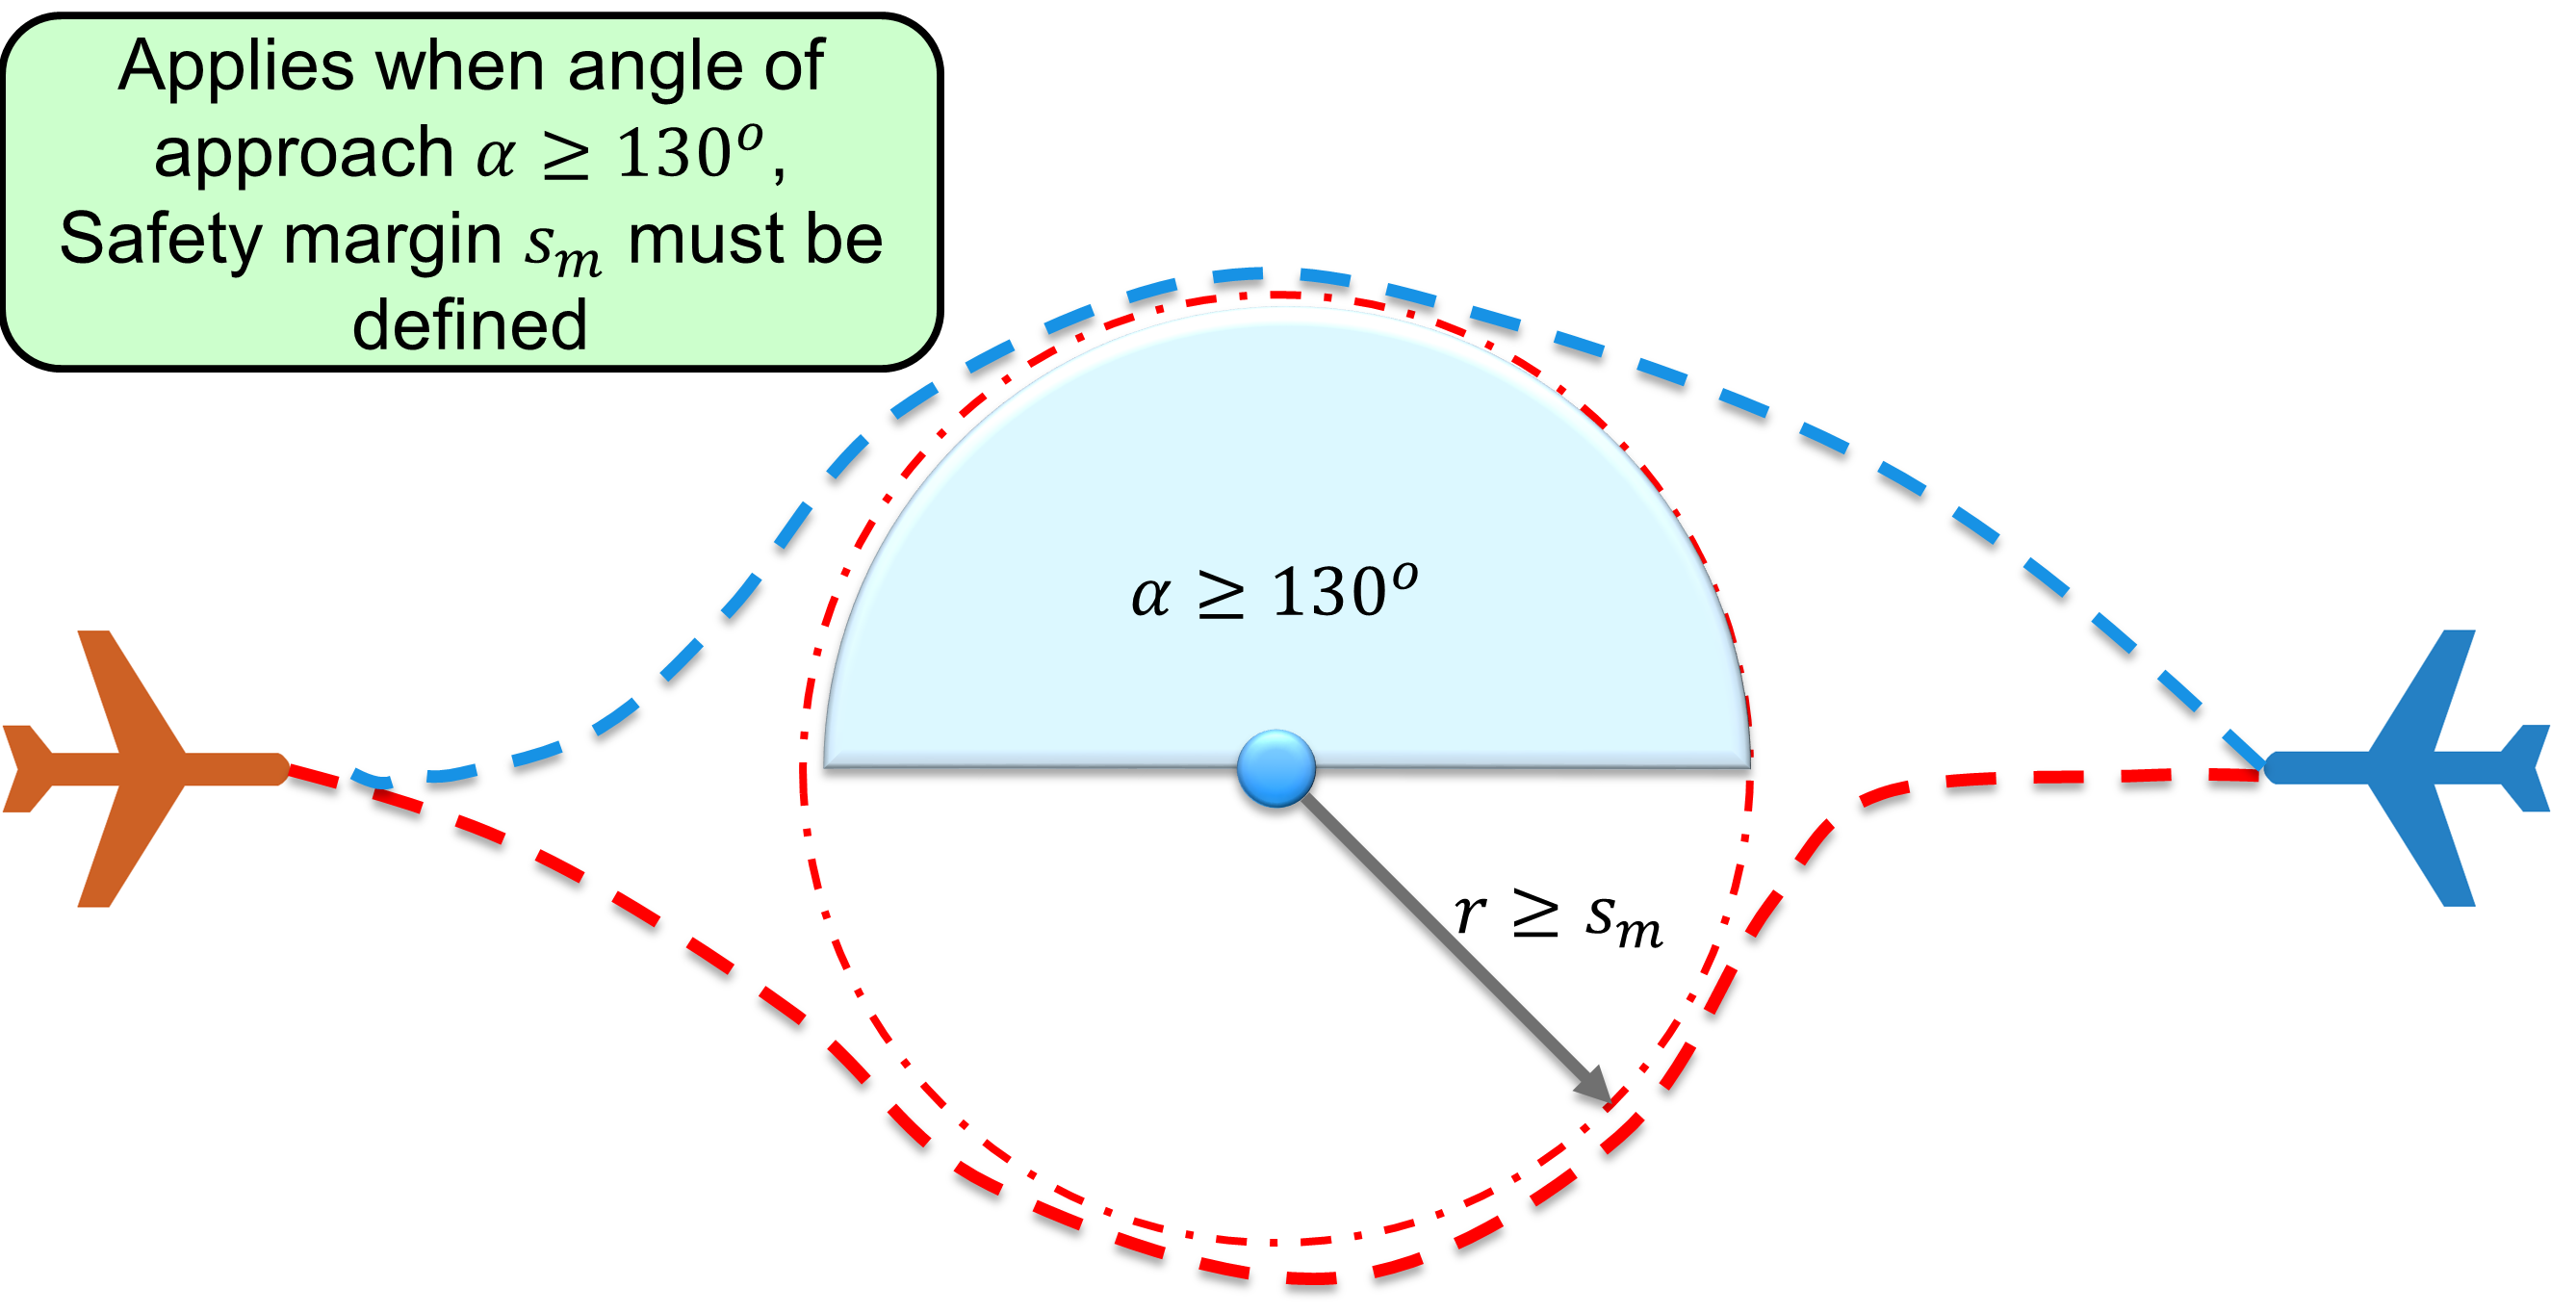
\includegraphics[width=0.9\linewidth,height=95pt,keepaspectratio]{\FIGDIR/RE008HeadOnApproach01} 
        \caption{Detection.}
        \label{fig:HeadOnApproachTheoreticalDetection}
    \end{subfigure}
    \begin{subfigure}{0.45\textwidth}
    	\centering
        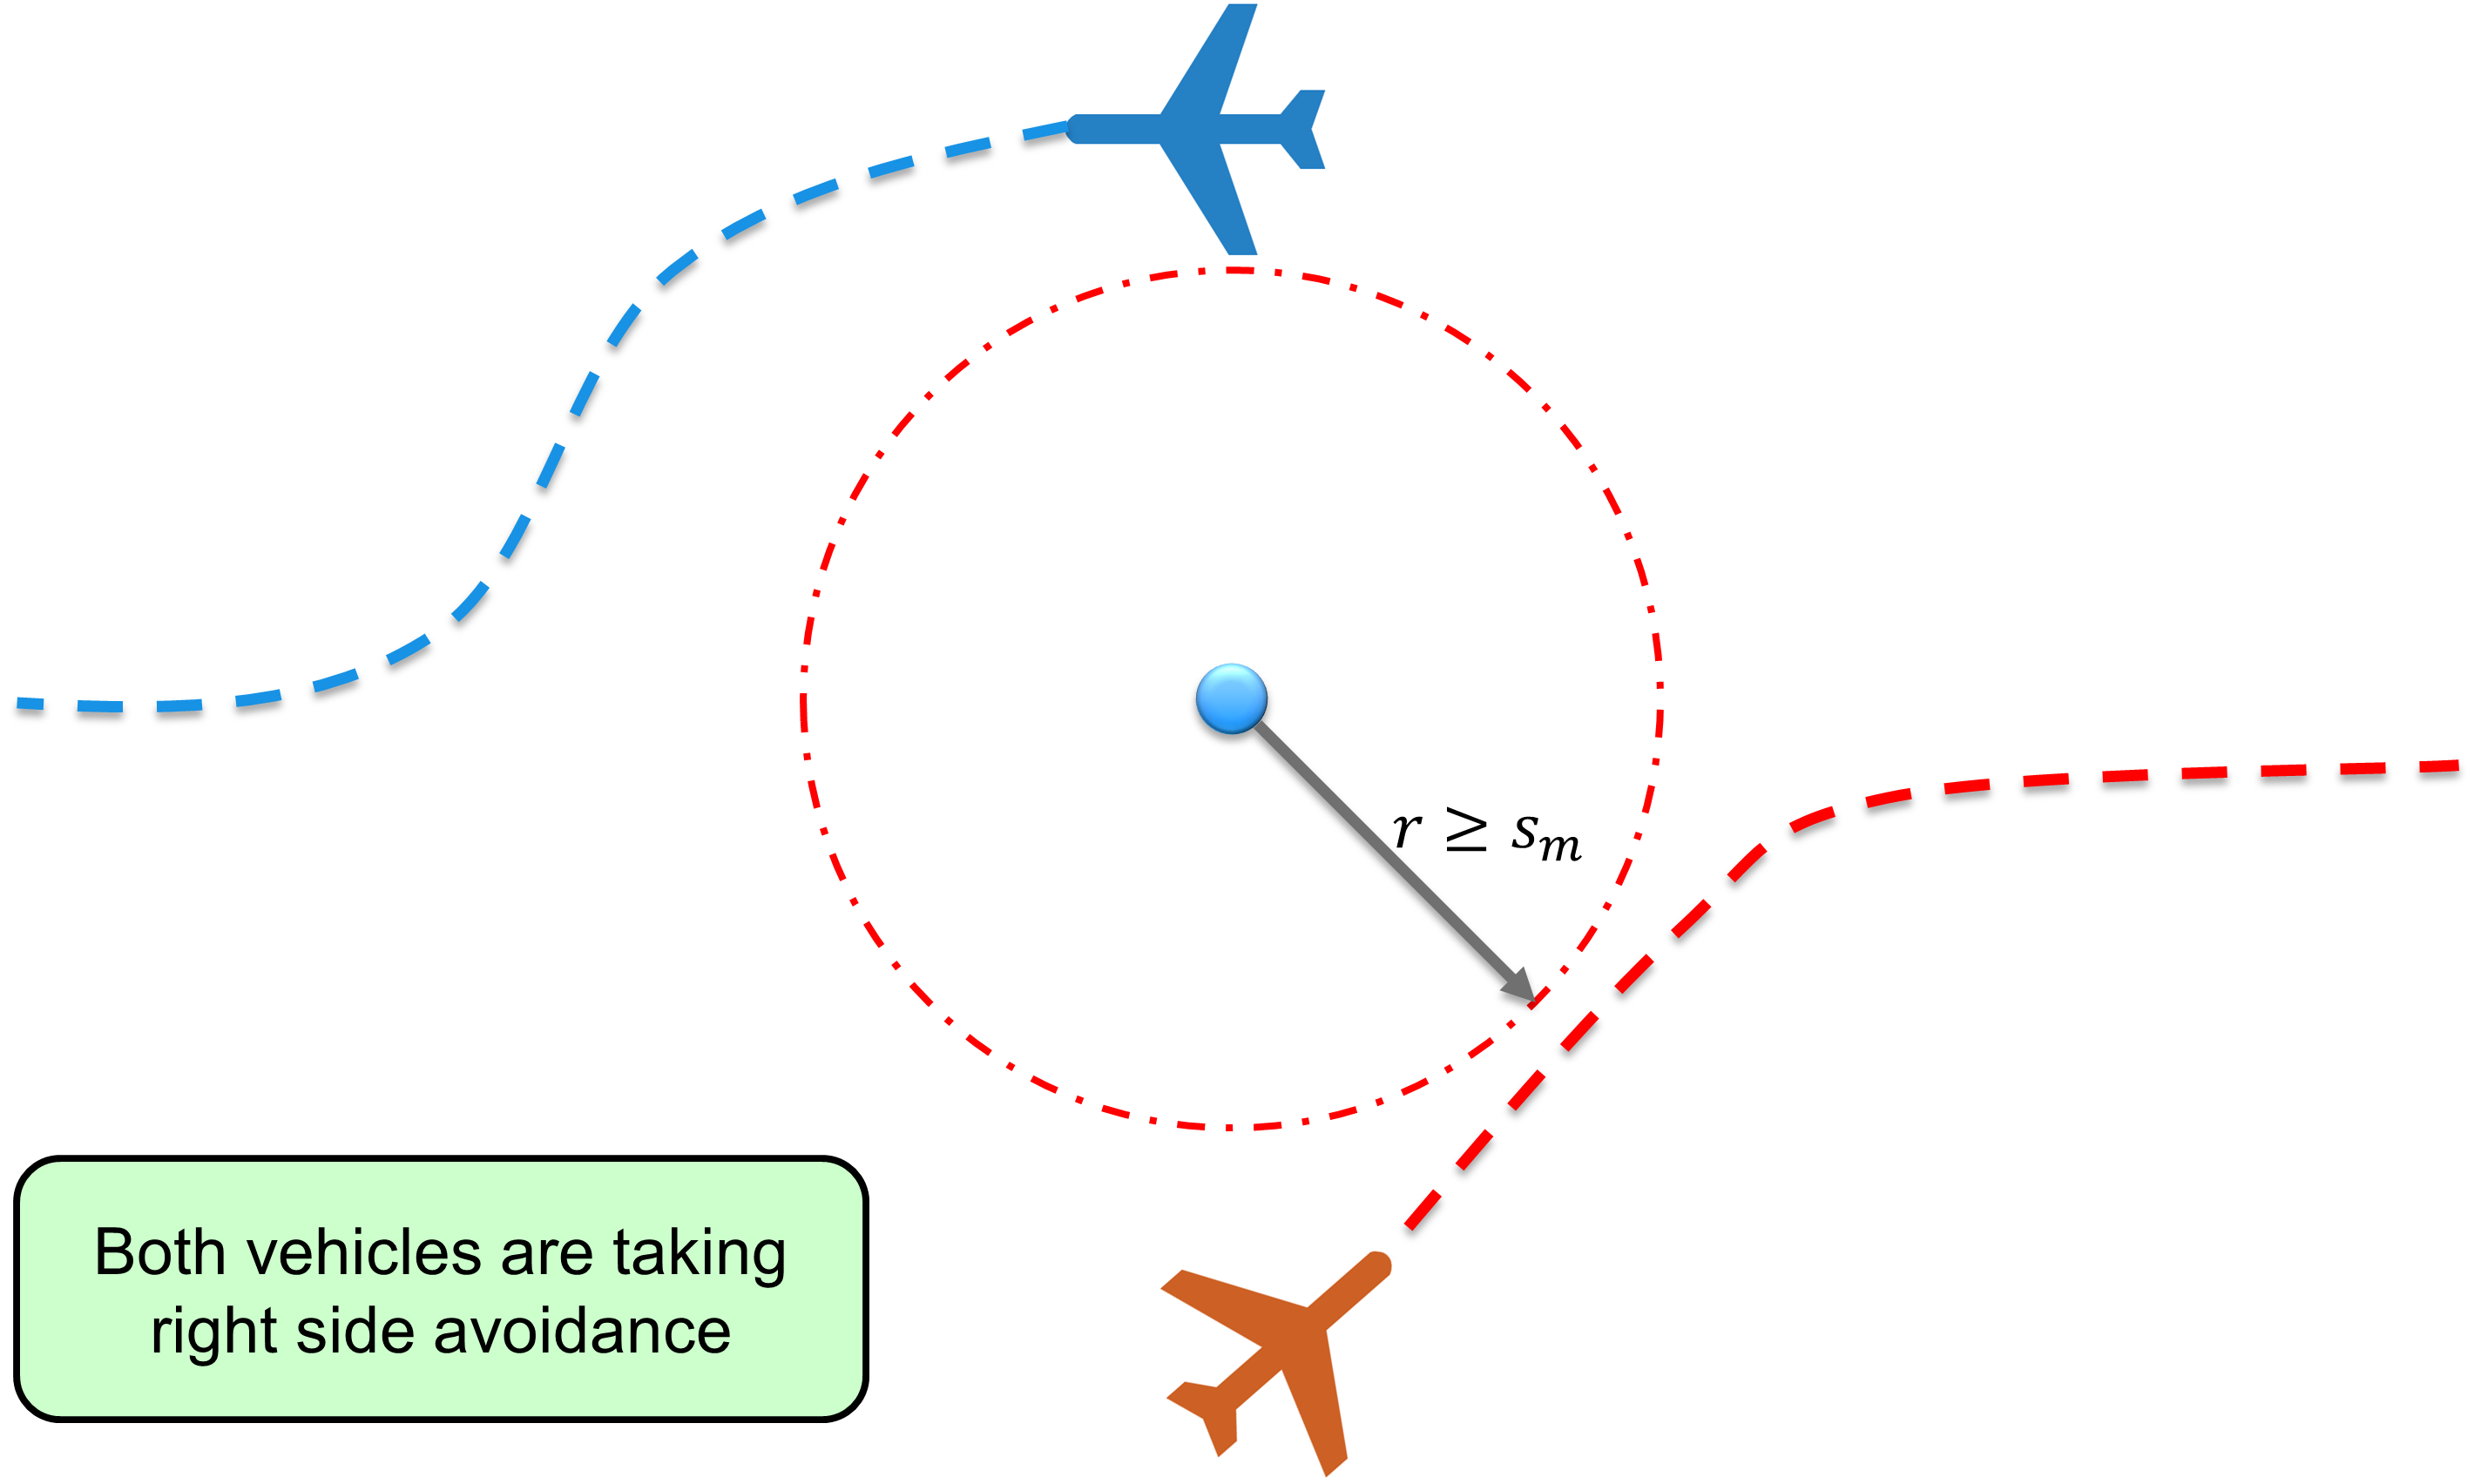
\includegraphics[width=0.9\linewidth,height=95pt,keepaspectratio]{\FIGDIR/RE009HeadOnApproach02} 
        \caption{Resolution/Closing.}
        \label{fig:HeadOnApproachTheoreticalResolution}
    \end{subfigure}
    \caption{Head-on approach detection/resolution/Closing}
    \label{fig:HeadOnApproachTheoretical}
\end{figure}

\paragraph{Triggering Events:} The \emph{head-on approach} (fig. \ref{fig:HeadOnApproachTheoretical}) \emph{triggering events} are the following:
\begin{enumerate}
    \item \emph{Detection} (fig. \ref{fig:HeadOnApproachTheoreticalDetection}) - the \emph{collision case} is open when \emph{collision point} with the respective angle of approach is detected. This must happen until the \emph{point of no return} is achieved. 
    
    \item \emph{Resolution} (fig. \ref{fig:HeadOnApproachTheoreticalResolution}) - the \emph{virtual} roundabout is enforced until the closing condition is met. 
    
    \item \emph{Closing} (fig. \ref{fig:HeadOnApproachTheoreticalResolution}) - based on the condition that all vehicles are heading away from \emph{collision point} and their mutual heading is neutral or opposite.
\end{enumerate} 

\paragraph{Virtual roundabout:} The \emph{flight levels} can be abstracted as the  \emph{virtual 2D surface}. The \emph{airspace attendants} are moving on virtual routes which can cross each other. The idea is to create virtual roundabout with enforced velocity to enable smooth collision avoidance.

\begin{enumerate}
    \item \emph{Center} - the center defined in \emph{airspace cluster} local coordinate system (flight level defining the horizontal placement).
    
    \item \emph{Diameter} - the minimal distance to \emph{center}, accounting the \emph{wake turbulence} and other phenomena. 
    
    \item \emph{Enforced velocity} - all attendants at \emph{virtual roundabout} keeps the same velocity. It helps to keep constant mutual distances.
\end{enumerate}



\subsection{\secState{R}Handling Converging Maneuver}\label{sec:handlingConvergingManuever}

\paragraph{Goal:} Identify \emph{required parameters} sufficient for automatic solution of \emph{Converging Maneuver}.

\paragraph{VFR:} The \emph{Visual Flight Rules} (VFR) are specified in annex 2 \cite{icaoAnnex2}. The rule is different from \emph{Head-on Approach} (sec. \ref{sec:handlingHeadOnApproach}) because multiple roles are depending on the relative aircraft position:
\begin{enumerate}
    \item \emph{Avoiding Aircraft} - there is an aircraft on the relative right side (blue). 
    \item \emph{Right Of the Way (ROA) Aircraft} - there is an aircraft on the relative left side (red). 
\end{enumerate}

The \emph{avoiding aircraft} should take the \emph{right of the way aircraft} from behind, with sufficient \emph{safety margin}, and return to original \emph{heading} afterward. The \emph{magnitude} of \emph{avoidance curve} must consider \emph{wake turbulence} and other impacts of \emph{avionic properties}.

\begin{note}
    This rule is applied only when both \emph{aircraft} belong to the same  \emph{maneuverability class} \cite{icaoAnnex2}.
\end{note}

\paragraph{IFR:} The \emph{Instrument Flight Rules} in annex 2. \cite{icaoAnnex2} and 11. \cite{icaoAnnex11} are defining \emph{converging maneuver} in detail.

The \emph{parameters} from a \emph{head-on approach} can be reused:
\begin{enumerate}
    \item $70^\circ$ $\le$ the \emph{Angle of Approach} $<$ $130^\circ$ - the minimal planar angle between aircraft position and expected collision point is in the interval $[70^\circ , 130^\circ[$.
    
    \item\emph{Minimal detection range} - given as $turning Radius + safety Margin$, while \emph{safety margin} is accounting all impact factors. 
    
    \item\emph{Safety margin} - during avoidance all aircraft keeps mutual distance at least on the value of \emph{Safety Margin}.
\end{enumerate}

\begin{note}
The lesser \emph{angle of approach} induces stronger wake turbulence impact on avoiding aircraft. This results in an increase of \emph{safety margin}. 

The \emph{wake turbulence} is represented as a droplet at the back of the plane. \emph{Wake turbulence range} can be calculated based on wake turbulence cone.
\end{note}

\begin{figure}[H]
	\centering
    \begin{subfigure}{0.32\textwidth}
    	\centering
        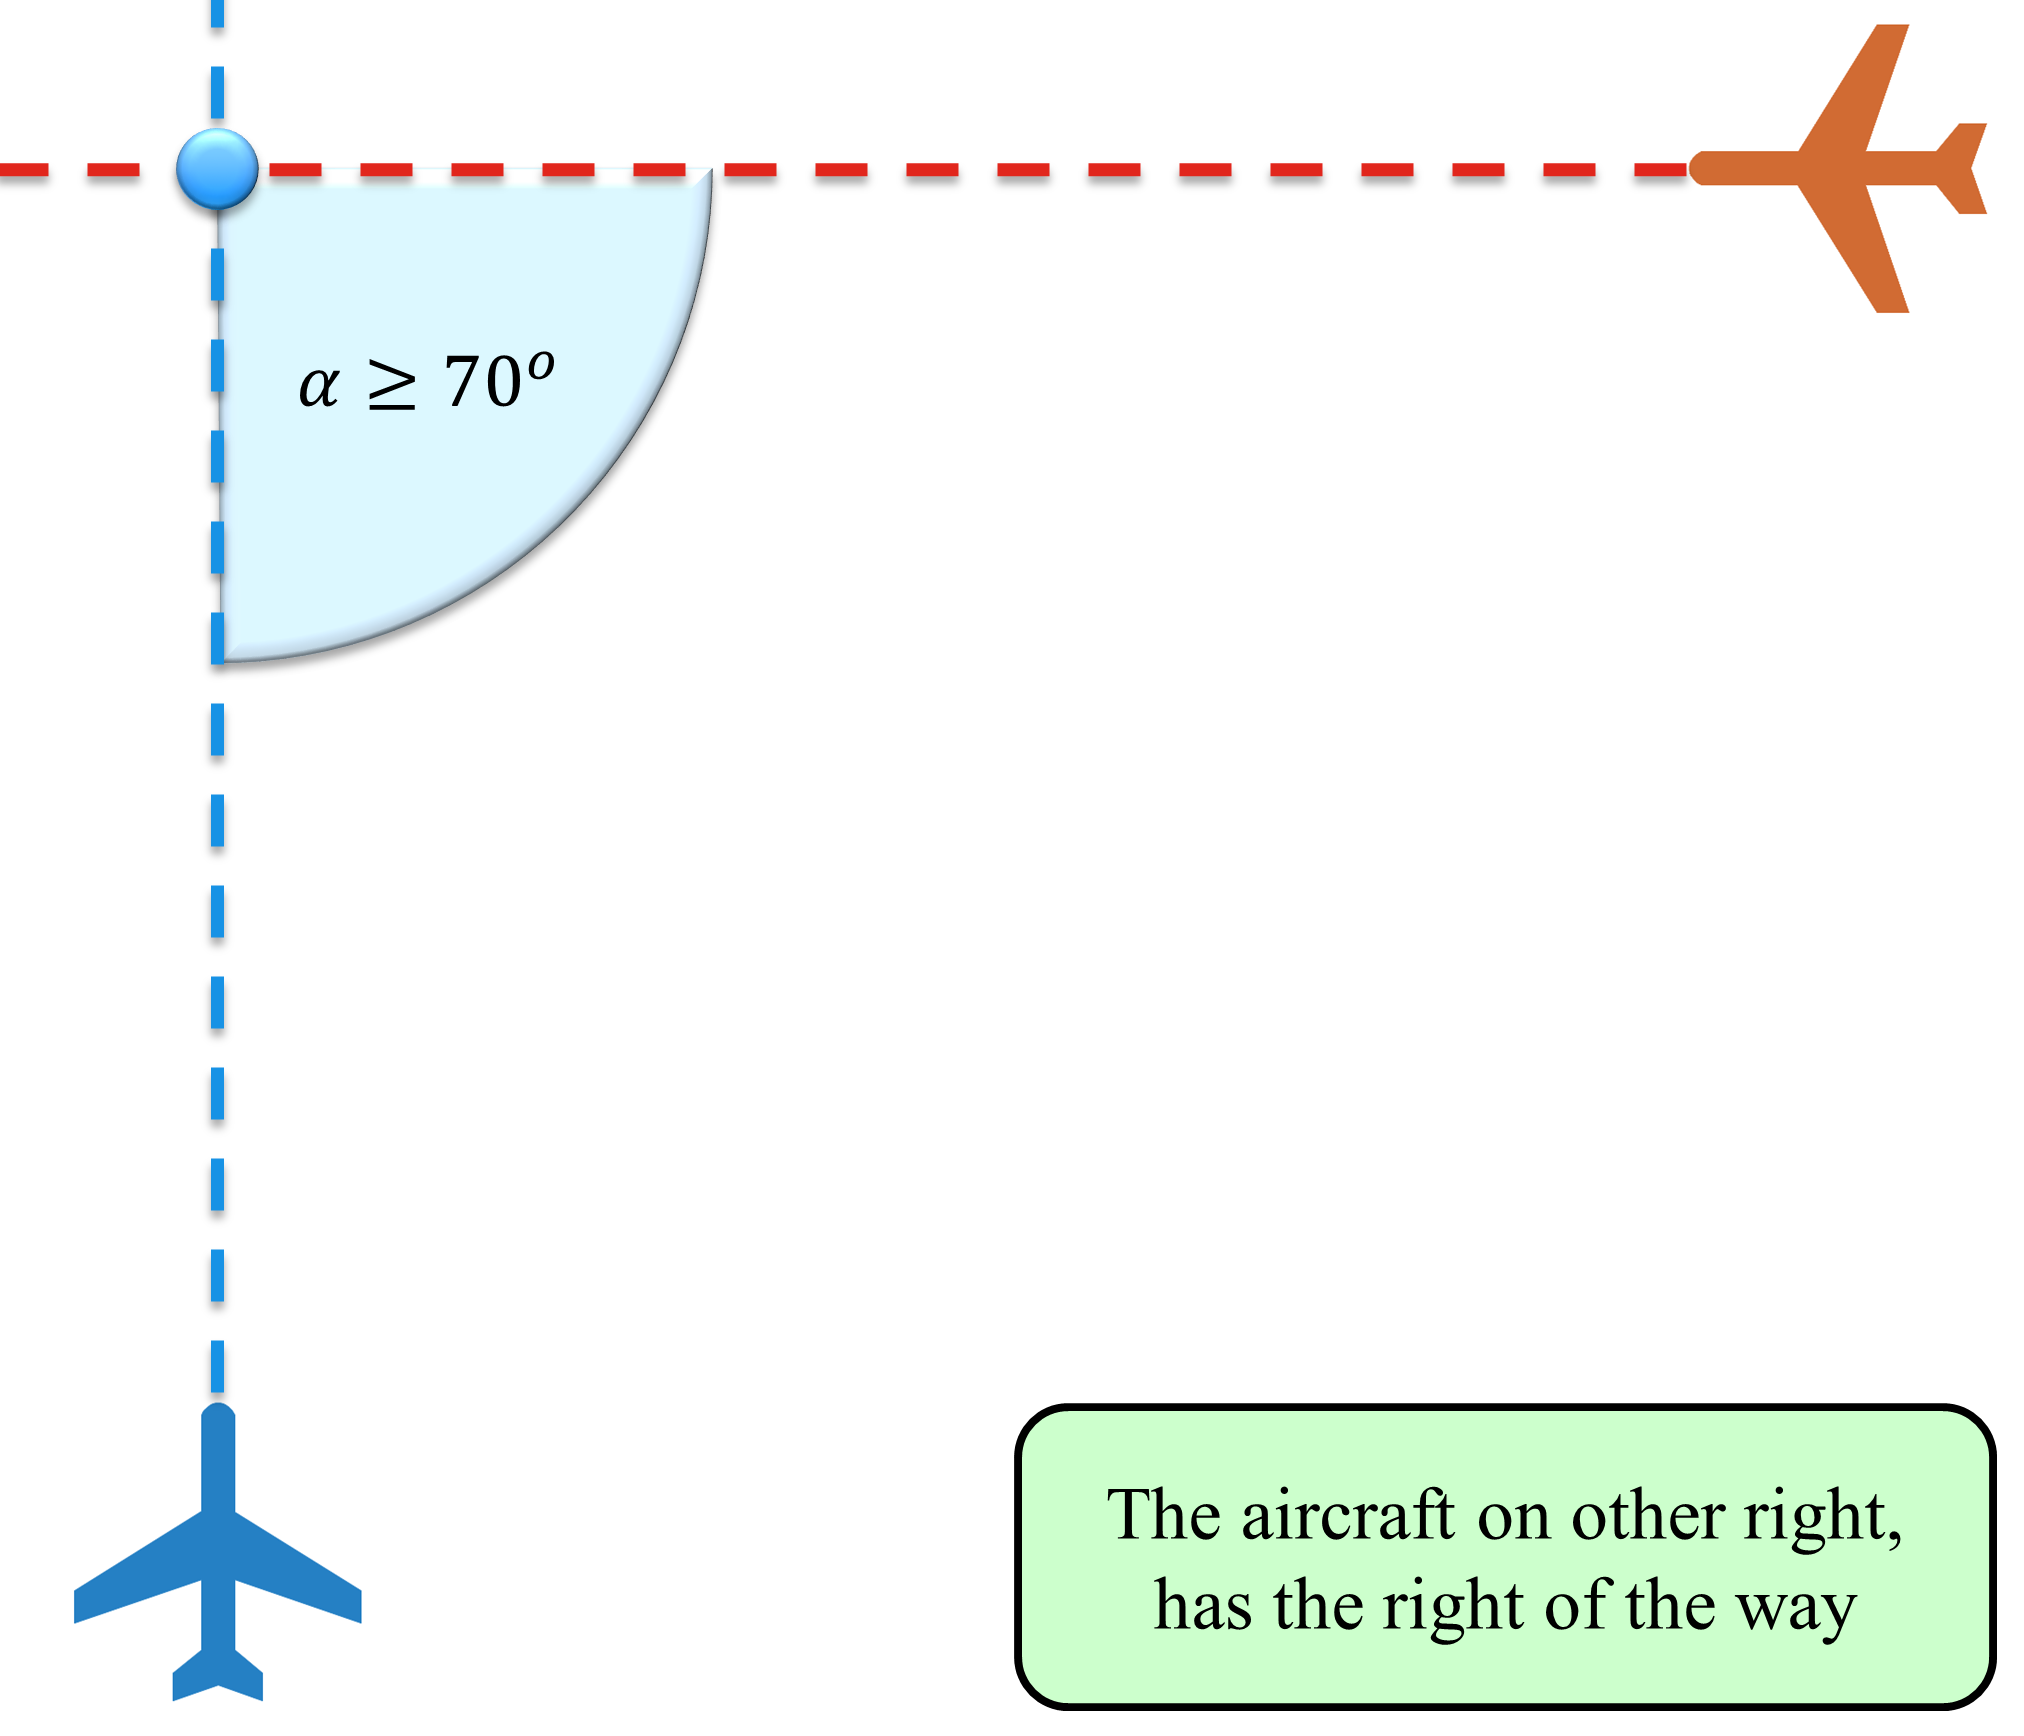
\includegraphics[width=0.9\linewidth,height=105pt,keepaspectratio]{\FIGDIR/RE005ConvergingManeuver01} 
        \caption{Detection.}
        \label{fig:ConvergingManeuverTheoreticalDetection}
    \end{subfigure}
    \begin{subfigure}{0.32\textwidth}
        \centering
        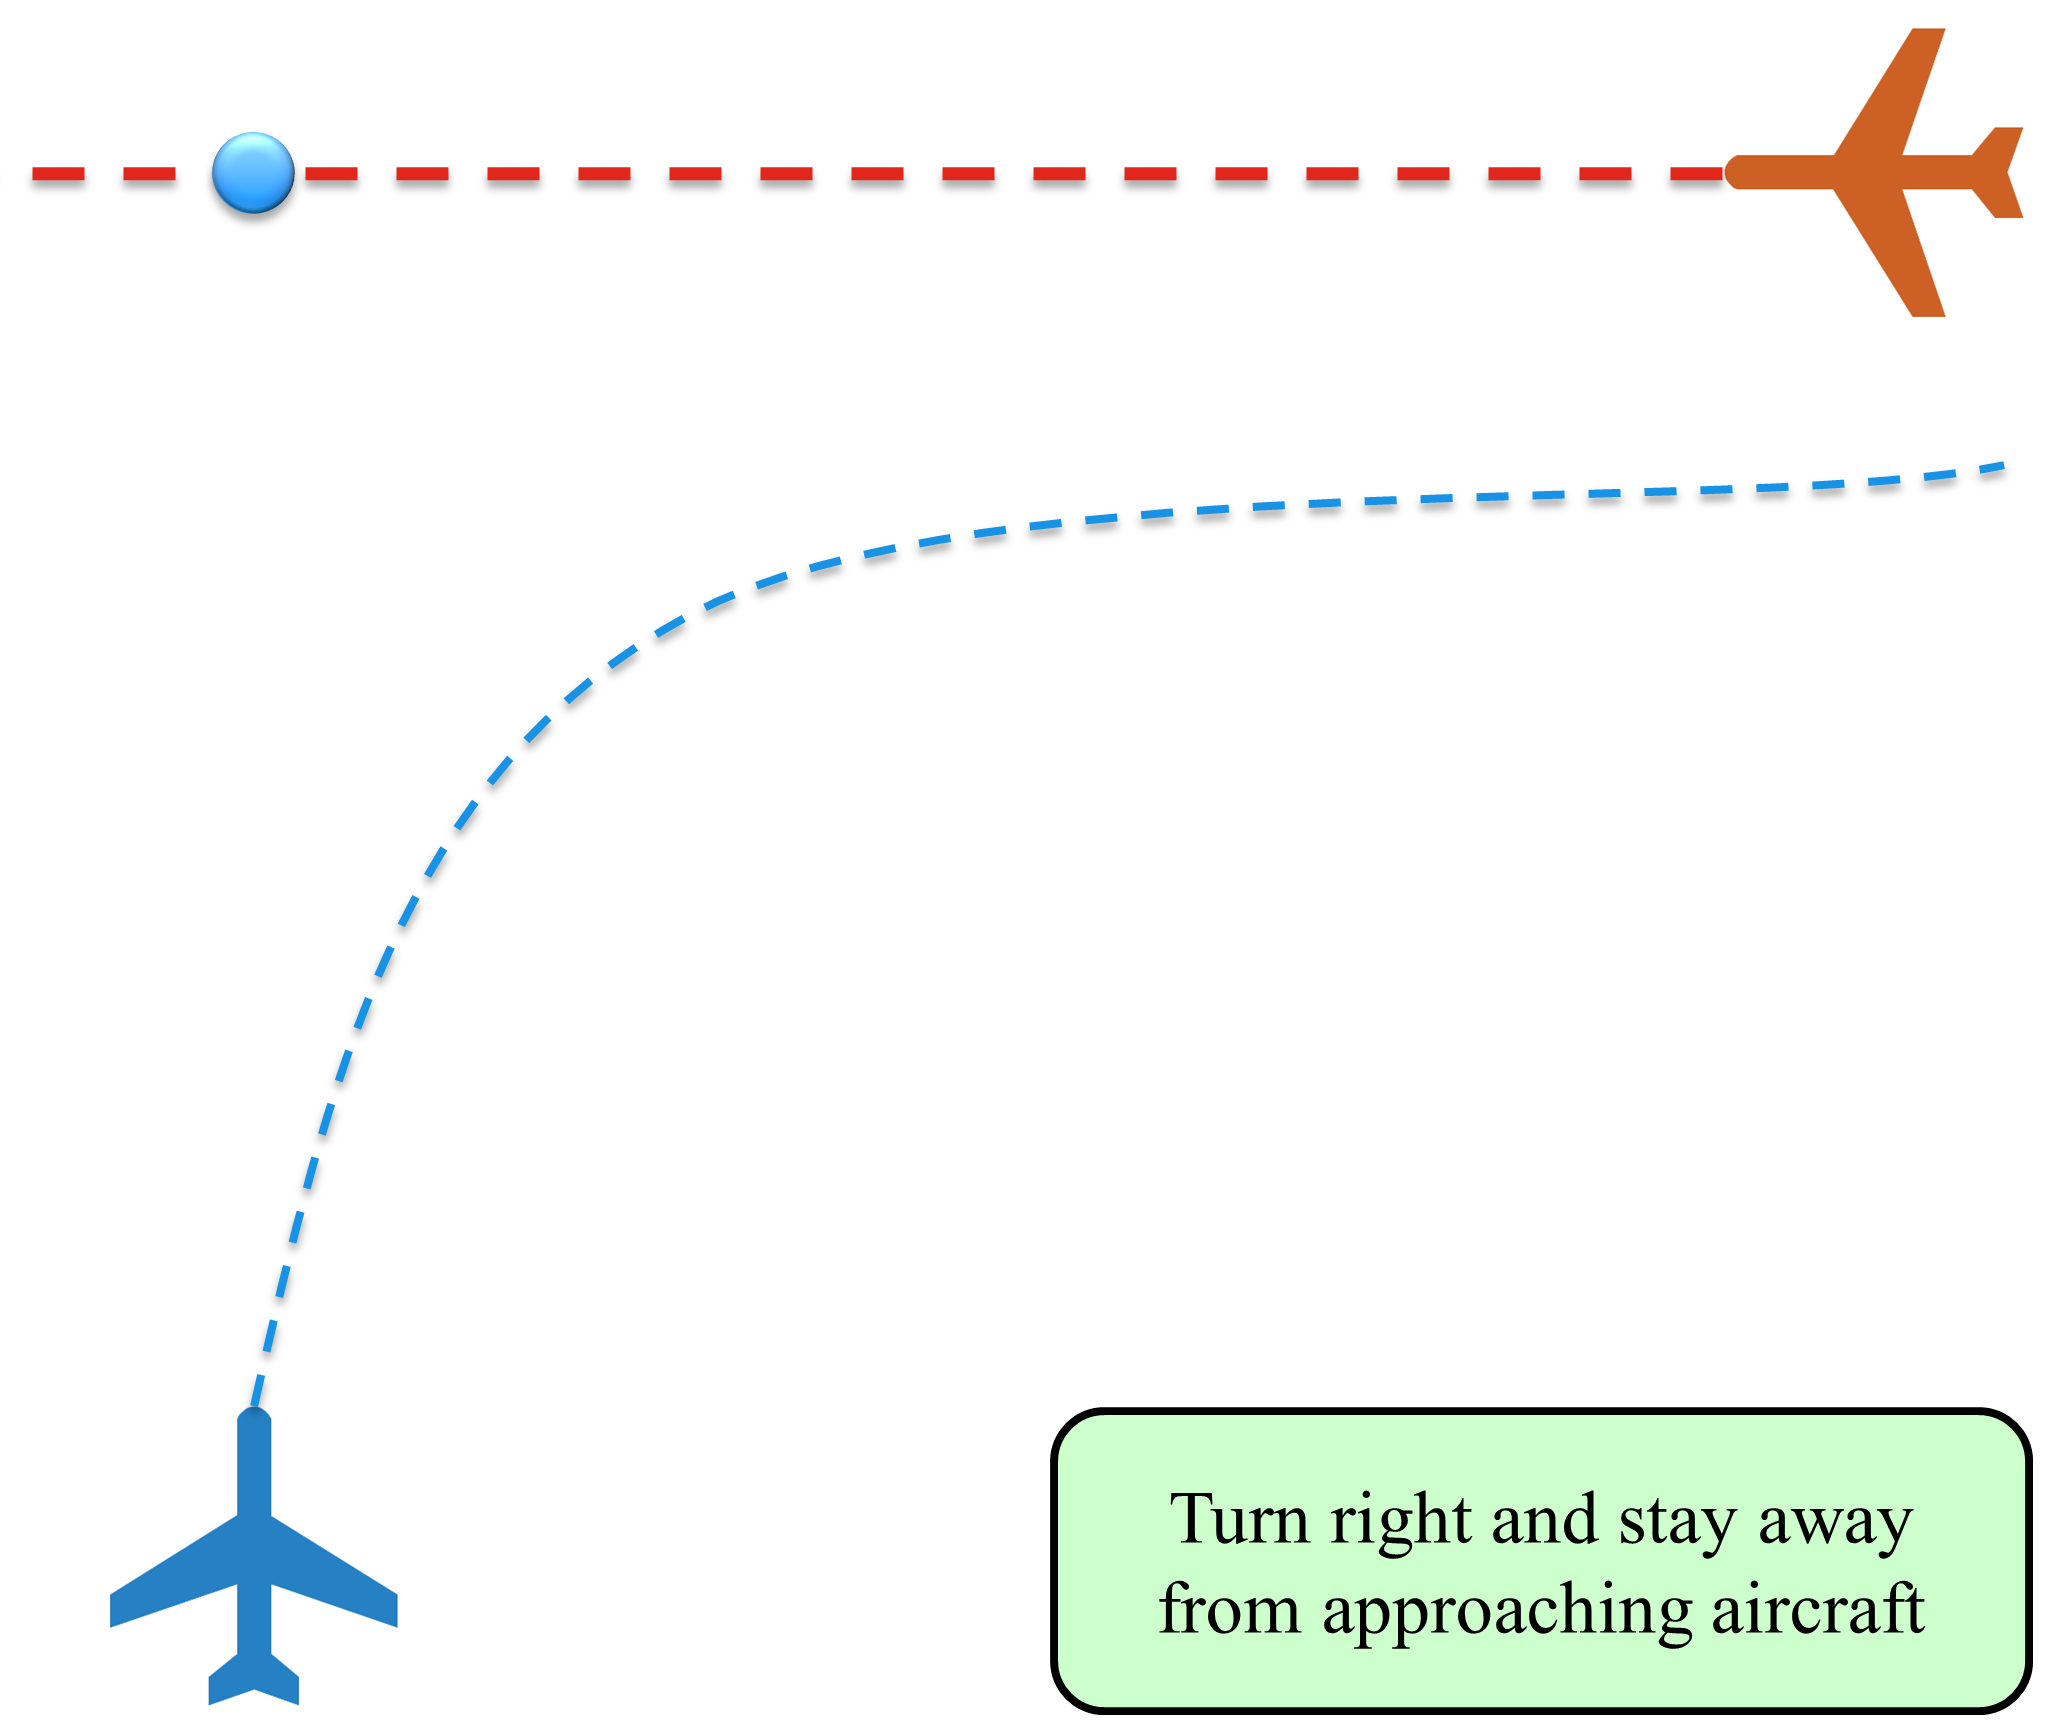
\includegraphics[width=0.9\linewidth,height=105pt,keepaspectratio]{\FIGDIR/RE006ConvergingManuever02} 
        \caption{Resolution.}
        \label{fig:ConvergingManeuverTheoreticalResolution}
    \end{subfigure}
    \begin{subfigure}{0.32\textwidth}
        \centering
        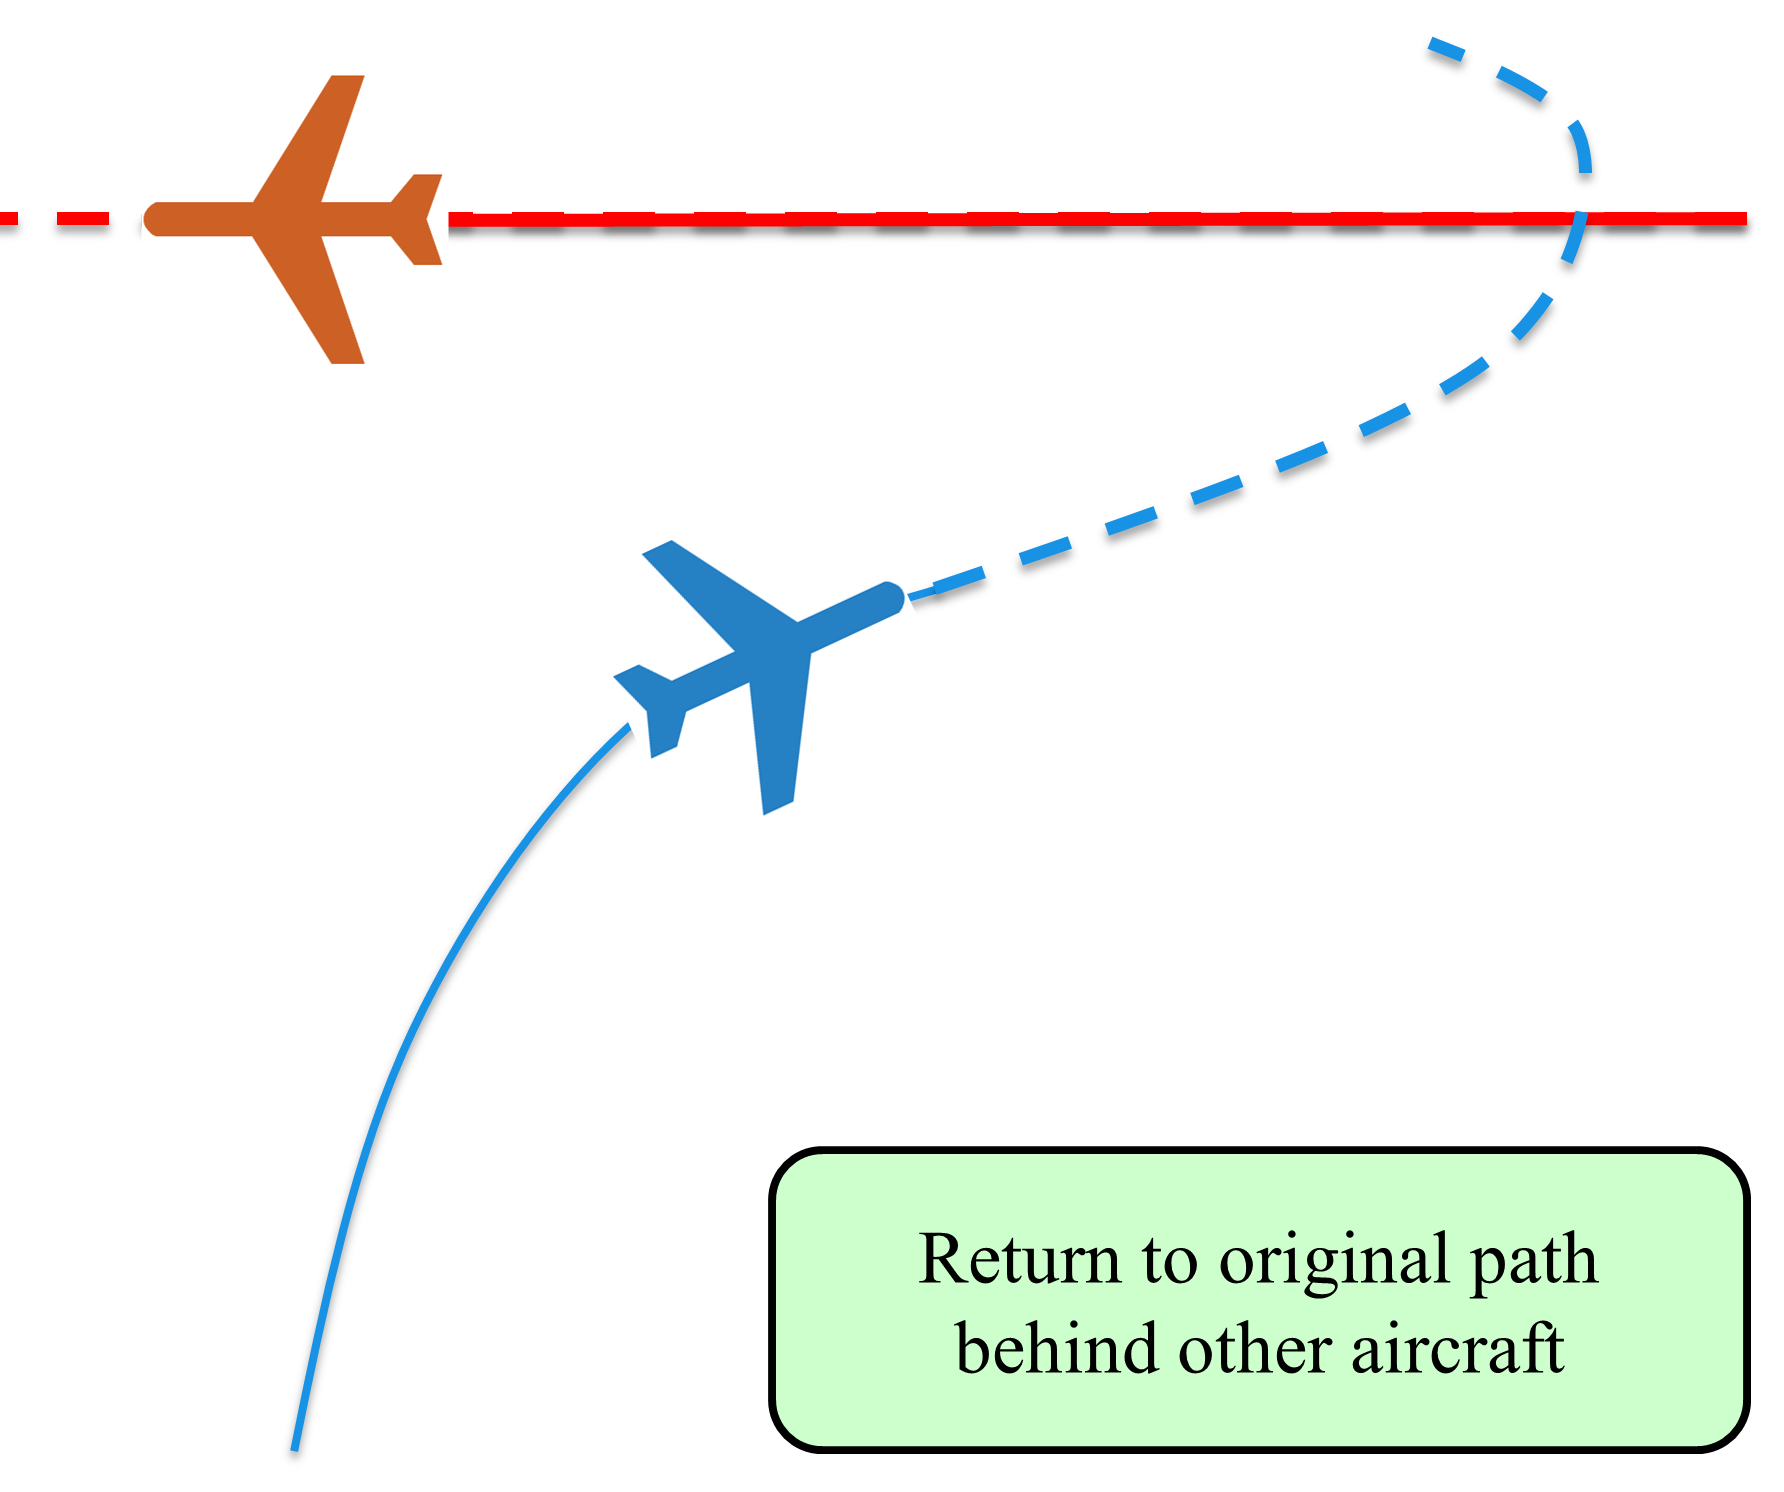
\includegraphics[width=0.9\linewidth,height=105pt,keepaspectratio]{\FIGDIR/RE007ConvergingManuever03} 
        \caption{Closing}
        \label{fig:ConvergingManeuverTheoreticalClosure}
    \end{subfigure}
    \caption{Converging maneuver Detection/Resolution/Closing}
    \label{fig:ConvergingManeuverTheoretical}
\end{figure}

\paragraph{Triggering Events:} The \emph{converging maneuver} (fig. \ref{fig:ConvergingManeuverTheoretical}) \emph{triggering events} are the following:

\begin{enumerate}
    \item \emph{Detection} (fig. \ref{fig:ConvergingManeuverTheoreticalDetection}) -  The \emph{avoiding airplane} (blue) detects \emph{collision point} (blue circle) which satisfy the \emph{converging maneuver conditions}. The distance between \emph{aircraft position} and \emph{collision point} is lesser than the \emph{detection range}.
    
    \item \emph{Resolution} (fig. \ref{fig:ConvergingManeuverTheoreticalResolution}) - the \emph{Right Of the Way aircraft} (red) stays at the original course. The \emph{avoiding aircraft} (blue) follows the \emph{parallel} to another \emph{plane}. The distance of \emph{avoiding plane} to \emph{other plane trajectory} is greater or equal to \emph{safety margin}.
    
    \item \emph{Closing} (fig. \ref{fig:ConvergingManeuverTheoreticalClosure}) - when both planes have an opposite heading, and they miss each other the converging maneuver can be closed. The \emph{avoiding airplane} will return to \emph{original trajectory}  while keeping the distance from \emph{another plane} (red) at greater or equal to \emph{safety margin}.
\end{enumerate}


\subsection{\secState{R}Handling Overtake Maneuver}\label{sec:handlingOvertakeManuever}

\paragraph{Goal:} Identify \emph{required parameters} sufficient for automatic solution of \emph{Overtake Maneuver}

\paragraph{VFR:} The \emph{Visual Flight Rules} (VFR) are specified in annex 2 \cite{icaoAnnex2}. The rule states that faster air traffic attendant may overtake slower one, from right side keeping sufficient distance (\emph{safety margin}). There are two forced roles:

\begin{enumerate}
    \item \emph{Overtaking} - faster aircraft with similar heading cruising in similar altitude than \emph{overtaken} (blue). It is expected that \emph{faster aircraft} has maneuvering capability to avoid slower aircraft.
    
    \item \emph{Overtaken} - slower aircraft which keeps the \emph{Right of the way}
\end{enumerate}

\begin{note}
    This rule is applied only when both aircraft have the same maneuverability class \cite{icaoAnnex2}. The overtake is considered \emph{borderline emergency maneuver} in controlled airspace because the aircraft tend to keep similar velocity in similar cruising altitude. The overtake is usual in \emph{non-controlled airspace}.
\end{note}

\begin{figure}[H]
	\centering
    \begin{subfigure}{0.32\textwidth}
        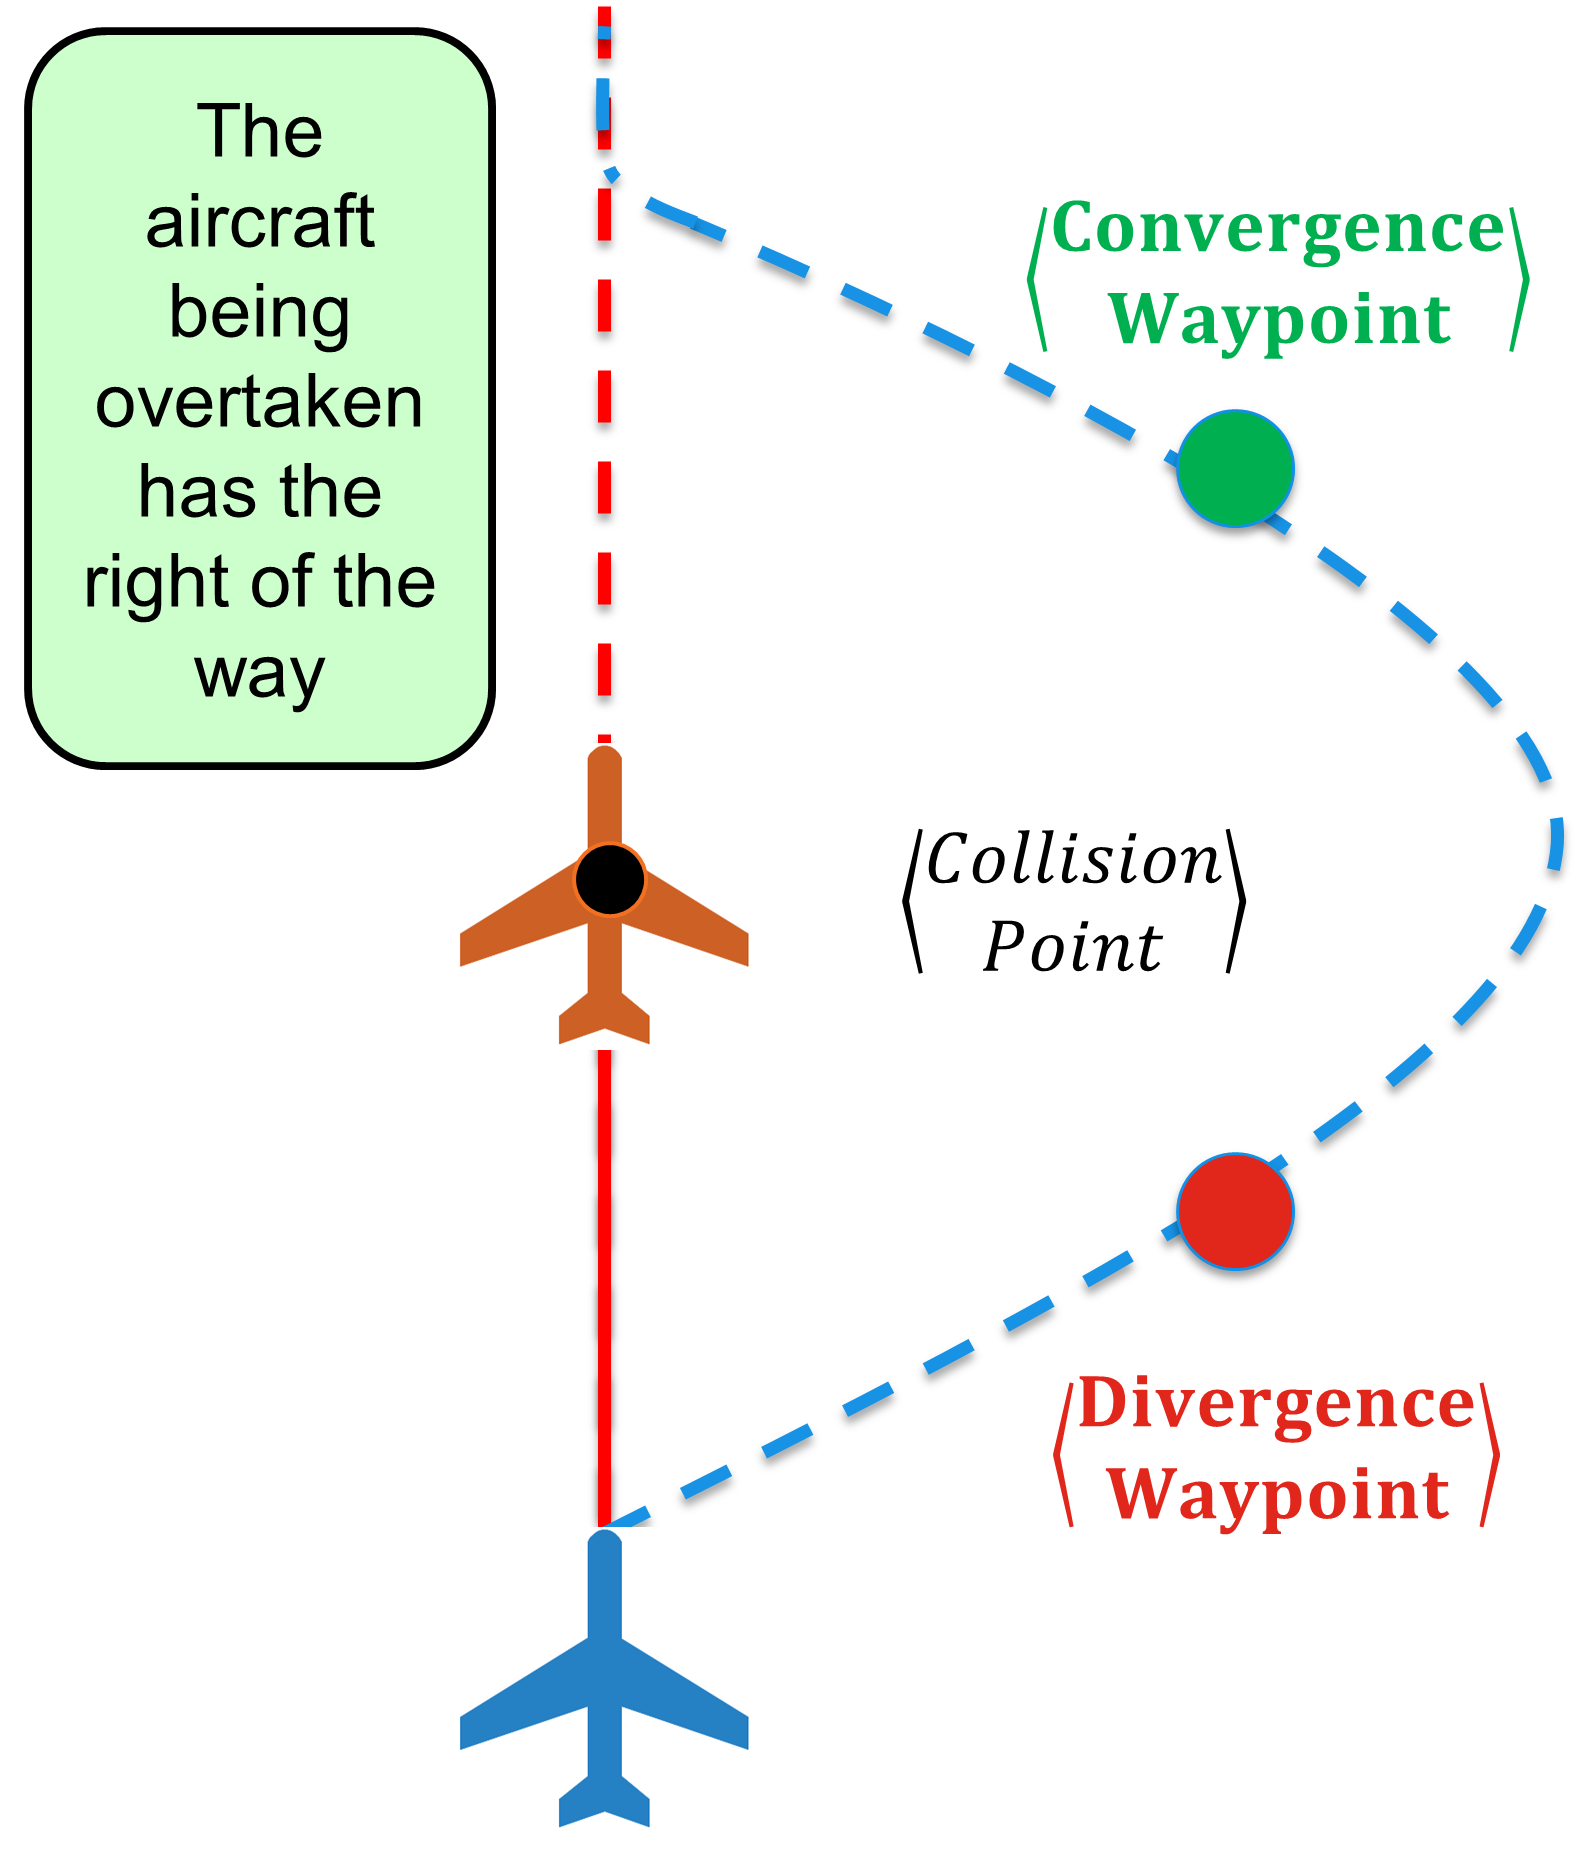
\includegraphics[width=0.9\linewidth,height=142pt,keepaspectratio]{\FIGDIR/RE010OvertakeMAnuever01} 
        \caption{Detection.}
        \label{fig:OvertakeManeuverTheoreticalDetection}
    \end{subfigure}
    \begin{subfigure}{0.32\textwidth}
        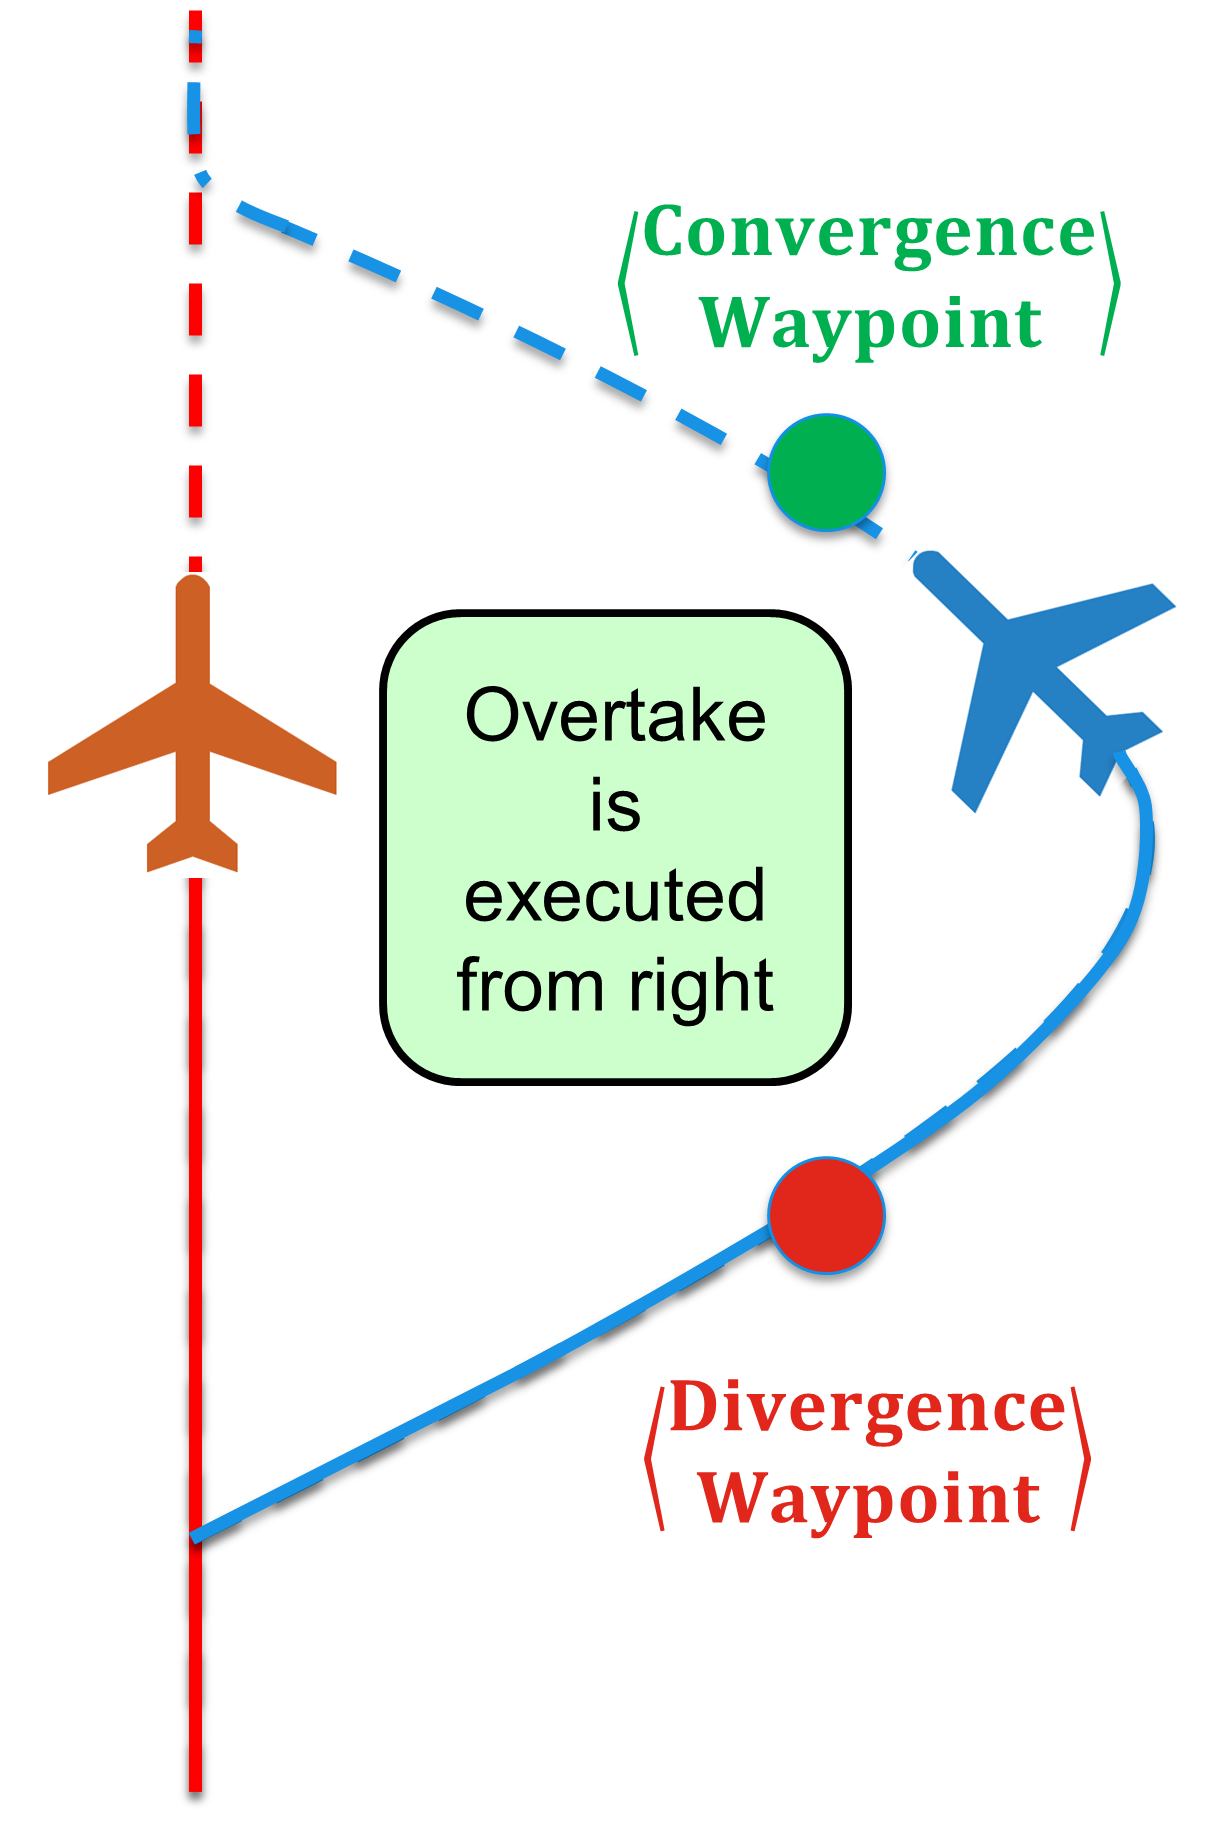
\includegraphics[width=0.9\linewidth,height=142pt,keepaspectratio]{\FIGDIR/RE011OvertakeMAnuever02} 
        \caption{Resolution.}
        \label{fig:OvertakeManeuverTheoreticalResolution}
    \end{subfigure}
    \begin{subfigure}{0.32\textwidth}
        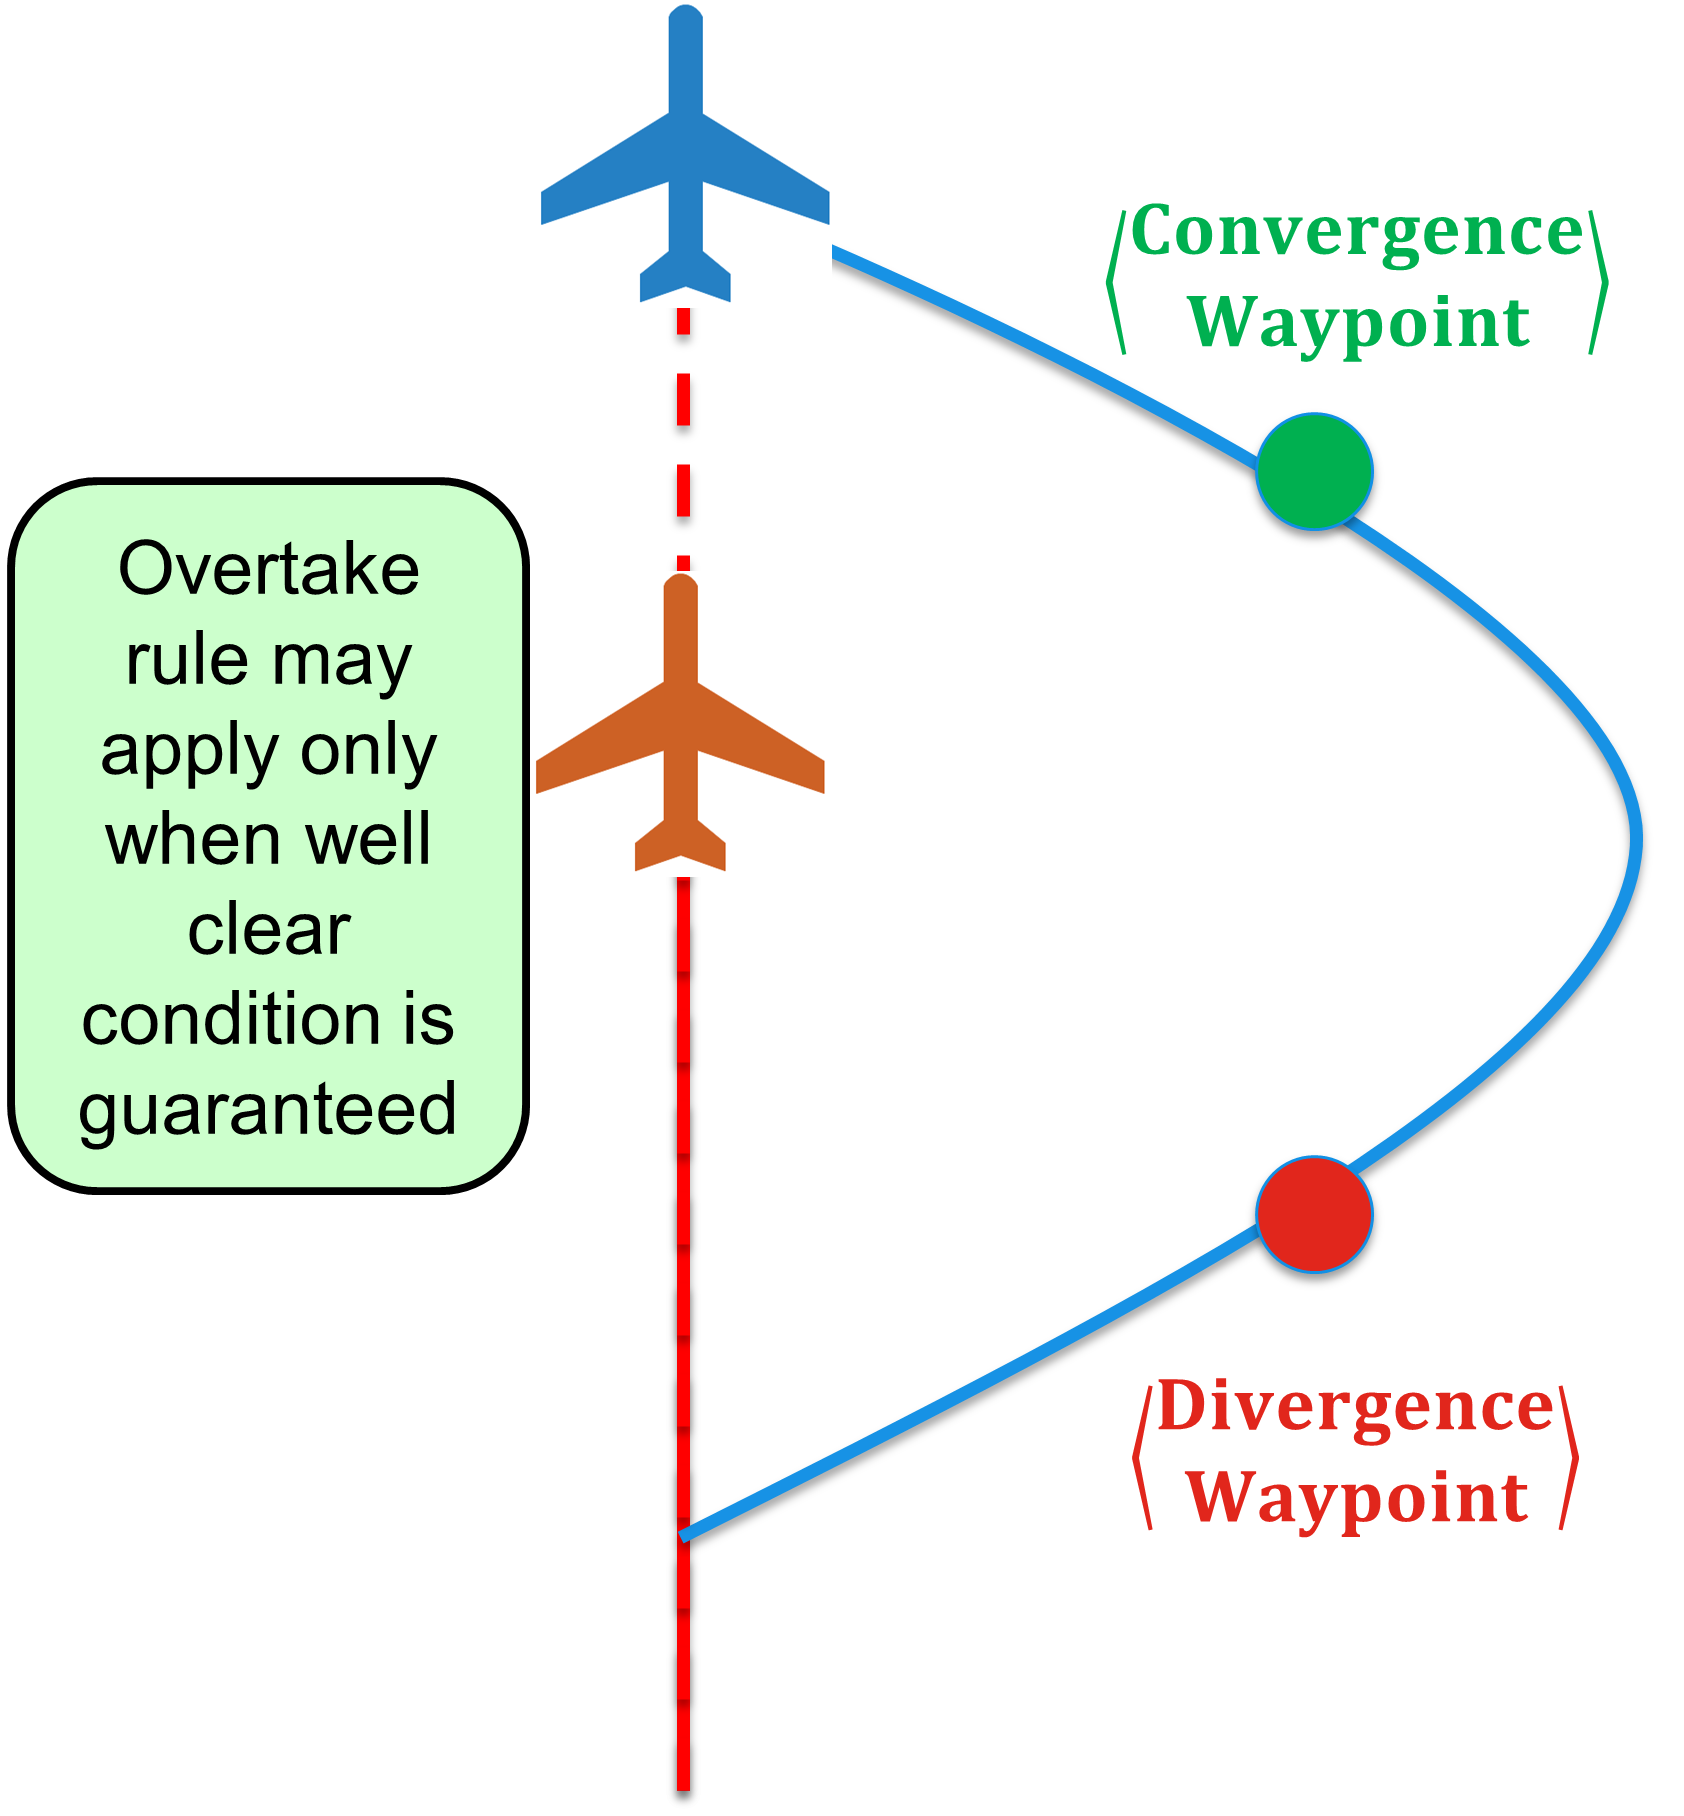
\includegraphics[width=0.9\linewidth,height=142pt,keepaspectratio]{\FIGDIR/RE012OvertakeMAnuever03} 
        \caption{Closing.}
        \label{fig:OvertakeManeuverTheoreticalClosure}
    \end{subfigure}
    \caption{Overtake maneuver Detection/Resolution/Closing}
    \label{fig:OvertakeManeuverTheoretical}
\end{figure}

\paragraph{IFR:} The \emph{Instrument Fight Rules} in annex 2. \cite{icaoAnnex2} and 11. \cite{icaoAnnex11} are defining the converging manual in detail:

\begin{enumerate}
    \item 0$^\circ \le$ the \emph{Angle of Approach} $<$ 130$^\circ$ - the minimal planar angle between aircraft position and expected collision point is in the interval $[0^\circ,70^\circ[$
    
    \item \emph{Minimal Detection Range} - given as $2 \times  reaction Time \times speed Difference$. 
    
    \item \emph{Safety Margin} - during avoidance the overtaking aircraft keeps the minimal distance of \emph{wake turbulence} of overtaken aircraft in own flight altitude. 
\end{enumerate}

\begin{note}
    The \emph{Safety Margin} is sufficiently small because speed difference is usually much lesser than in case of  \emph{Head-on approach}. The \emph{Wake turbulence} can be avoided completely by taking the higher altitude level than overtaken aircraft.
\end{note}


\paragraph{Triggering events:}
\begin{enumerate}
    \item \emph{Detection} (fig. \ref{fig:OvertakeManeuverTheoreticalDetection}) - occurs when the distance between \emph{overtaking} (blue) and overtaken (red) is approaching \emph{minimal detection range} or double of \emph{safety margin}. If the performance of \emph{overtaking aircraft} (blue) allows taking \emph{sharp right side to overtake} the \emph{Maneuver starts}, otherwise \emph{overtaking aircraft} (blue slows down) and keeps at least \emph{safety margin distance} to avoid \emph{wake turbulence}.
    
    \item \emph{Resolution} (fig. \ref{fig:OvertakeManeuverTheoreticalResolution}) - \emph{overtaken} (red) is keeping same heading and \emph{speed} during overtake maneuver. The \emph{overtaking} (blue) projects two waypoints: \emph{Divergence} and \emph{Convergence} keeping the required separation minimum during overtake. Then the \emph{overtaking} (blue) diverges heading to \emph{Divergence waypoint}. When the \emph{Divergence waypoint} is reached by \emph{overtaking} (blue) aircraft, it changes to \emph{original heading}.
    
    \item \emph{Closing} (fig. \ref{fig:OvertakeManeuverTheoreticalClosure}) - the \emph{closing} of \emph{Overtake} starts when \emph{overtaking} aircraft (blue) have sufficient lead over \emph{overtaken} aircraft (red). The \emph{overtaking} aircraft (blue) can safely change the heading to the original waypoint.
\end{enumerate}


\paragraph{Constant Cruising Speed:} Most of the traffic attendants at same flight level have similar (close to constant) cruising speed. Lower flight levels are for slower turbo-prop planes, and higher altitudes are for jet planes. It is stated that this principle will persist even when UAS will be integrated \cite{bayen2005langrangian,kopardekar2002dynamic,helme1992optimization} in multiple air-traffic models.


